\chapter{Programmentwurf}
Auf einer abstrakte Ebene kann das Programm wie folgt beschrieben werden (vgl. Abbildung \ref{sse}):
Ein Parser liest die Daten der Classifier über das Bild aus einer CSV Datei aus und speichert die Daten der Relationen in den \textit{Relation} Objekten und die Daten über die Primitive in den \textit{Primitive} Objekten. Der Parser hält eine Liste all dieser Objekte. Die Anwendung holt sich die Daten der Relation Objekte. Jedes Relation Objekt enthält seine zwei zugehörigen Primitive Objekte. Dadurch werden alle Primitive, die nicht Teil einer Relation sind von nun an nicht weiter verwendet.\
Zunächst berechnet die Relation eine Tabelle mit der akkumulierten Evidenz zu jedem Primitiv. Danach generiert sie eine akkumulierte Tabelle mit der Evidenz aus den beiden Primitiven. Diese wird in einem \textit{Solution} Objekt festgehalten. Nun kann ein \textit{Relation} Objekt mithilfe seines zugehörigen \textit{Solution} Objekt Schilder generieren.

\begin{figure}[htbp]
    \centering
    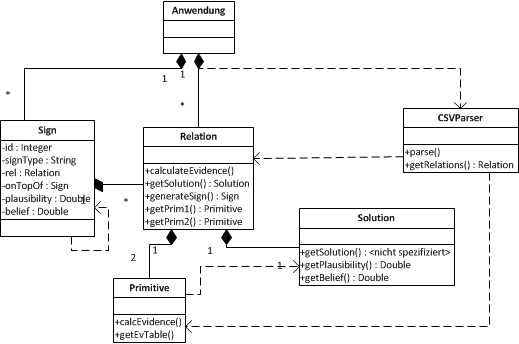
\includegraphics[scale=1]{images/uml.png}
    \caption{UML Diagram der StreetSign Evidence Anwendung}
    \label{sse}
\end{figure}

Ergibt sich daraus ein Schild, wird dieses in einer Liste gespeichert. Nachdem Relationen auf Schilder überprüft wurden, wird geprüft, ob eine Relation zwei Schilder in eine örtliche Relation zu bringen. Für jede \textit{on top} Relation wird geprüft, ob deren erstes und zweites Primitiv ein gültiges Schild enthält. Wenn diese Bedingung erfüllt wird, merkt sich das örtlich obere Schild, dass und welches Schild sich unter ihm befindet.\
\
Am Ende wird über alle Schilder iteriert und ausführlich die bekannten Informationen zu den erkannten Schildern ausgegeben.


